\subsection{Magnetic Field Interpolation} \label{ssec:prop_magfield}
    \begin{figure}[ht] % Note: Maybe a pie chart would be better for this?
        \centering
        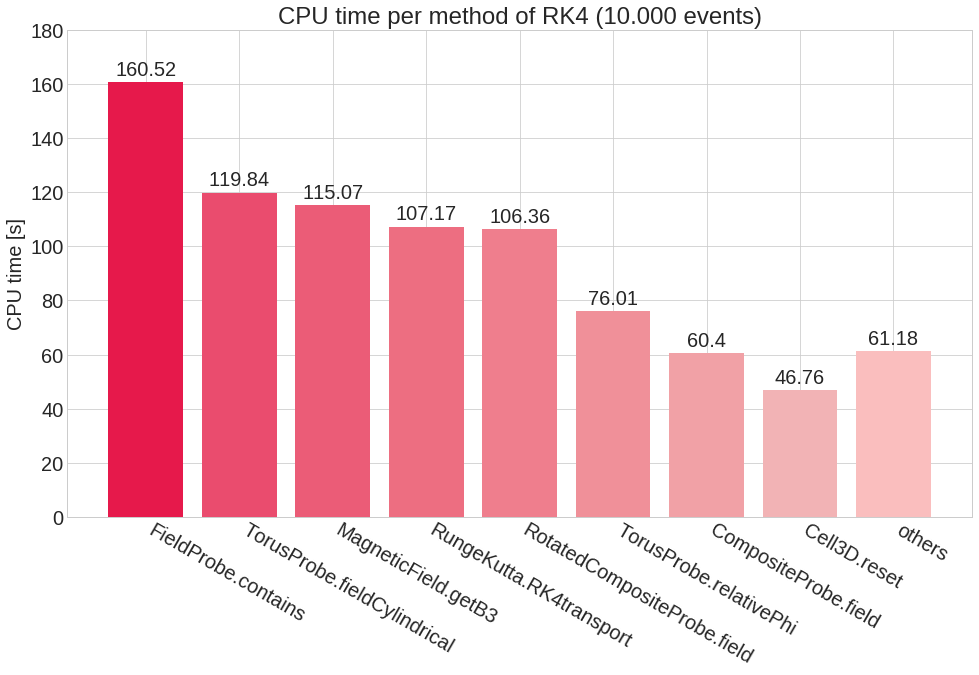
\includegraphics[scale=0.44]{bfield/rk4_composition}
        \caption{\label{fig:rk4_composition} CPU times consumed by each Runge Kutta 4 component.}
    \end{figure}

As seen in Figure \ref{fig:rk4_composition}, most of the Runge Kutta 4 algorithm's runtime is actually used by methods retrieving the magnetic field from the \texttt{swimmer} package.
These methods' purposes is to compute the magnetic field $\textbf{B}(x,y,z) = \langle \operatorname{B_1}(x,y,z),\operatorname{B_2}(x,y,z),\operatorname{B_3}(x,y,z)\rangle$ at a specific $(x,y,z)$ point inside the CLAS12 detector, which is done by placing virtual ``probes'' inside it. % Note: Maybe I should elaborate more on this.

To accelerate this computation, the possibility of using trilinear interpolation~\cite{bourke1999interpolation} for $\mathbf{B}$ was analyzed.
The option was considered favorable since the imprecision brought by interpolating the value instead of directly computing it could be diminished by the \textbf{update} part of the KF and by only using the interpolated magnetic field in a fixed number of iterations of the KF before using the real magnetic field for the remaining ones.
Appendix \ref{add:trilinear_interpolation} describes how trilinear interpolation works.

The algorithm used is a direct transcription of the definition of trilinear interpolation, and is defined in two steps.
First, obtain the regular grid and the measurements at each border, which is done by selecting a grid size $\left([\text{min}_x, \text{max}_x], [\text{min}_y, \text{max}_y], [\text{min}_z, \text{max}_z]\right)$ from which the magnetic field measurements are taken with step sizes defined as $\{\text{ss}_x, \text{ss}_y, \text{ss}_z\}$.
These parameters define a regular tridimensional grid and a measurement for the magnetic field for each point in this grid is obtained.

For the second step, the specific measurement in the location desired is obtained by evaluating the formula defined in \ref{add:trilinear_interpolation}.
In the case that the location is outside the range of the regular grid, the real magnetic field is computed for that point.

After the interpolation algorithm was implemented, the borders and the step size of the grid were left as parameters to be tuned.
First, $[\text{min}_z, \text{max}_z]$ were set to $[229 \text{cm}, 569 \text{cm}]$ since these are the limits of the $z$ variable in the detector.

    \begin{figure}[ht]
        \centering
        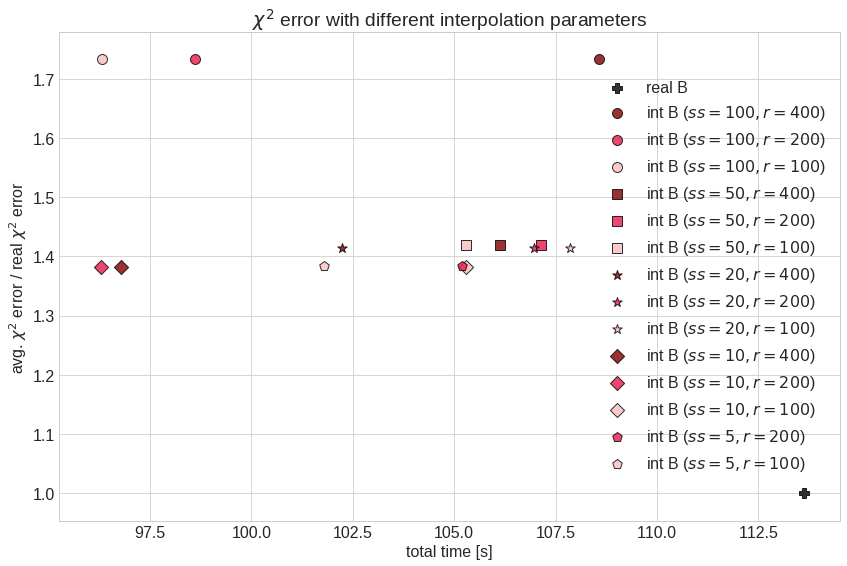
\includegraphics[scale=0.52]{bfield/chi2_vs_time}
        \caption{\label{fig:bfield_chi2_vs_time} $\chi^2$ error when doing the track fitting with the interpolated magnetic field divided by the obtained when using the real magnetic field vs required time. ``real B'' is the real magnetic field while ``int B'' is the interpolated magnetic field with its parameters in parentheses.}
    \end{figure}

To set the step size for each variable, $\text{ss}$ is defined such that $\text{ss} = \text{ss}_x = \text{ss}_y = \text{ss}_z$ for simplicity.
Then, the range $[\text{min}, \text{max}]$ and the variable $r$ are defined such that $\text{min} = \text{min}_x = \text{min}_y$ and $\text{max} = \text{max}_x = \text{max}_y$ and $r = \text{max} = \text{-min}$, to take advantage of the symmetries of the detector, which can be seen in Figures \ref{fig:dc_horizontal_cut} and \ref{fig:dc_vertical_cut} from Section \ref{ssec:framework_dc}.

Tests are ran by running the software using the interpolated magnetic field with different combinations of parameters, comparing them using the division of the $\chi^2$ error obtained by the one found when running the real field and measuring it against the time it takes to run the program.
The results are averaged over a set of $2.500$ estimated tracks and the results can be seen in Figure \ref{fig:bfield_chi2_vs_time}.
It is worth noting that some outliers are removed from the figure to aid with visualization.
The tested values for each were the following:
    \begin{align*}
        \text{ss} &\in \{5 \text{cm}, 10 \text{cm}, 20 \text{cm}, 50 \text{cm}, 100 \text{cm}, 200 \text{cm}\}\\
        r &\in \{100 \text{cm}, 200 \text{cm}, 400 \text{cm}\}
    \end{align*}

As seen in the figure, the interpolation parameters that provide the best results are $\text{ss} = 10 \text{cm}$ and $r = 200 \text{cm}$.

    \begin{figure}[ht]
        \begin{floatrow}
            \ffigbox[0.48\textwidth]{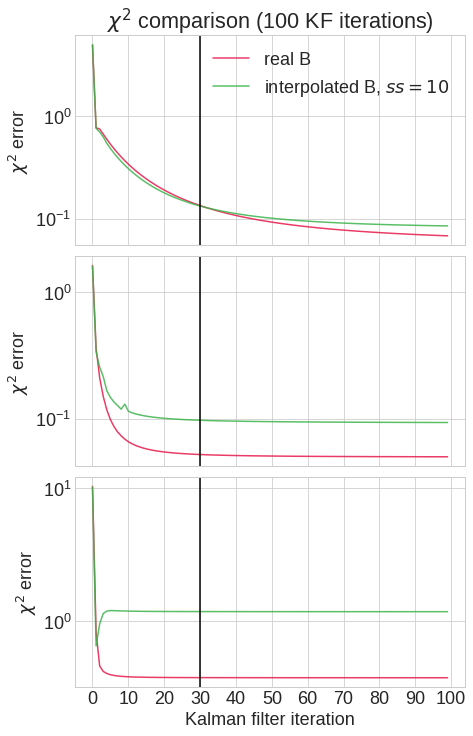
\includegraphics[height=0.72\textwidth] 
            {bfield/chi2_real_vs_ss10}}
                {\caption{\label{fig:bfield_real_vs_ss10} $\chi^2$ error comparison between real magnetic field and interpolated one with a step size of $10$ running the KF with $100$ iterations. A vertical black line denotes the $30$ usual KF iterations.}}
                
            \ffigbox[0.48\textwidth]{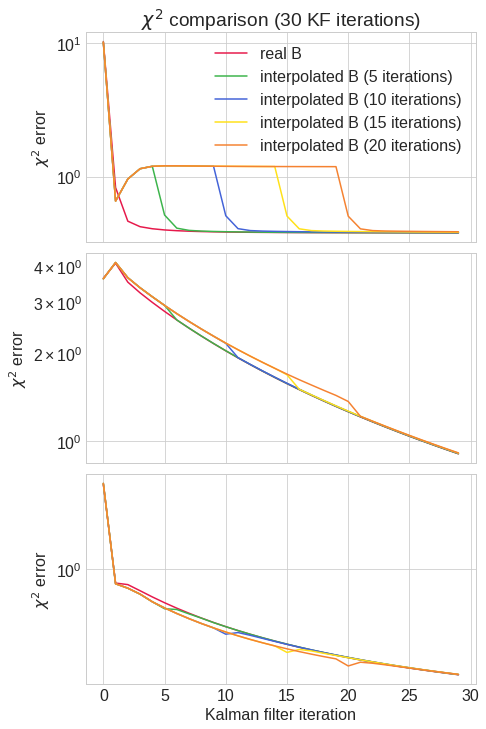
\includegraphics[height=0.72\textwidth] {bfield/chi2_real_vs_ni20}}
                {\caption{\label{fig:bfield_real_vs_ni20} $\chi^2$ error comparison between the real magnetic field and the interpolated one for different numbers of iterations running the KF with $30$ iterations.}}
        \end{floatrow}
    \end{figure}

Figure \ref{fig:bfield_real_vs_ss10} then shows the $\chi^2$ error of three distinct tracks running $100$ KF iterations, contrasting the error of the real magnetic field to that of the selected interpolated version.
As can be seen the figure, in most cases both version converge similarly but the one using the real magnetic field provides better results, albeit generally taking up more time.

Finally, a compromise that still provides good results is reached by running only the first KF iterations using the interpolated magnetic field and the last ones using the real one.
The number of iterations using the interpolated field tested are $0$, $5$, $10$, $15$, $20$, $25$ and $30$, but at the end all but the last one end up with the same final $\chi^2$ error.
Due to this, the number of interpolated magnetic field steps is decided based on the total DCHB and DCTB times when using each version, as presented in Table \ref{tab:interpolated_steps_times}.

It is worth noting that the total times per event listed here are slightly different than the ones presented in the validations of the method, and this is because these tests were ran on $3.000$ events instead of the usual $10.000$.
This decision is taken for the sake of expediency and because it shouldn't affect the results in a significant manner.

    \begin{table}[ht]
        \centering
        \begin{tabular}{@{}l|ll@{}}
        \toprule
        Name                  & DCHB time [s] & DCTB time [s] \\ \midrule
        Real magnetic field   & 130.42        & 48.78         \\
        5 interpolated steps  & 133.42        & 52.05         \\
        10 interpolated steps & 110.94        & 42.24         \\
        15 interpolated steps & 107.87        & 40.76         \\
        20 interpolated steps & 103.83        & 38.46         \\
        25 interpolated steps & 109.52        & 40.14         \\
        30 interpolated steps &  96.63        & 35.14         \\ \bottomrule
        \end{tabular}
        \caption{\label{tab:interpolated_steps_times} DCHB and DCTB times [s] using different interpolated steps.}
    \end{table}

As can be seen in Table \ref{tab:interpolated_steps_times}, the best times were obtained by running $30$ interpolated steps, but the final number of interpolated steps set in the code are $20$, the second best.
This decision is taken due to the fact that, as can be seen in Figure \ref{fig:bfield_real_vs_ni20}, if no steps are taken with the real magnetic field, the final $\chi^2$ error is much higher than the original one.
Figure \ref{fig:bfield_real_vs_ni20} shows the $\chi^2$ error obtained by using this method.

It's worth noting that the interpolation is only implemented in the Hit-Based tracking part of the KF since the Time-Based part requires as much precision as possible.
% Note: This could use a citation but it came from a meeting with Veronique. It's due to the fact that DCTB analyzes using a much finer grain than DCHB, and DCHB is mostly used to quickly filter tracks so that DCTB doesn't need to analyze all of them.